% =====================================================================
%  Pakistan ClimateTwin -- IEEE conference-format research paper
%  Compile on Overleaf (IEEEtran is built in): upload this folder as a zip,
%  set the compiler to pdfLaTeX, and click Recompile.
%
%  TODO for the team before submission:
%   * Replace the author block with your names, IDs and emails.
%   * Read the cited papers and extend Section II with your own reading.
%   * Rewrite any sentence you cannot explain in your own words.
% =====================================================================
\documentclass[conference]{IEEEtran}
\IEEEoverridecommandlockouts
\usepackage{cite}
\usepackage{amsmath,amssymb}
\usepackage{graphicx}
\usepackage{booktabs}
\usepackage{multirow}
\usepackage{xcolor}
\usepackage{url}
\usepackage{tikz}
\usetikzlibrary{positioning,arrows.meta}
\graphicspath{{figures/}}
\newcommand{\degC}{\ensuremath{^\circ}C}
\def\BibTeX{{\rm B\kern-.05em{\sc i\kern-.025em b}\kern-.08em T\kern-.1667em\lower.7ex\hbox{E}\kern-.125emX}}

\begin{document}

\title{A Machine Learning-Enabled Climate Digital Twin for Historical Climate Analysis and Short-Term Temperature Prediction in Pakistan Using Google Earth Engine}

\author{
\IEEEauthorblockN{Author One}
\IEEEauthorblockA{\textit{Dept. of Computer Science} \\
\textit{National University of Computer and Emerging Sciences}\\
City, Pakistan \\
email@example.com}
\and
\IEEEauthorblockN{Author Two}
\IEEEauthorblockA{\textit{Dept. of Computer Science} \\
\textit{National University of Computer and Emerging Sciences}\\
City, Pakistan \\
email@example.com}
\and
\IEEEauthorblockN{Author Three}
\IEEEauthorblockA{\textit{Dept. of Computer Science} \\
\textit{National University of Computer and Emerging Sciences}\\
City, Pakistan \\
email@example.com}
}

\maketitle

% ---------------------------------------------------------------------
\begin{abstract}
Pakistan is highly exposed to rising temperatures and heat extremes, yet district-level evidence on where and when warming occurs, and on how predictable monthly heat is, remains fragmented. We present Pakistan ClimateTwin, a research-scale climate digital twin built on Google Earth Engine (GEE). We extract monthly ERA5-Land temperature, soil moisture and radiation, CHIRPS v3 rainfall and SRTM elevation for 126 districts over 2000--2025 (39{,}312 district-months). Mann--Kendall tests with Sen's slope and false-discovery-rate control show that warming is mainly a night-time and monsoon-season phenomenon: national minimum temperature (Tmin) rose by +0.19\,\degC/decade, while maximum temperature (Tmax) shows no trend; the diurnal range shrank in 125 of 126 districts, and 12 districts, concentrated in Sindh and coastal Balochistan, are significant Tmin warming hotspots. Daytime trends depend strongly on elevation (Spearman $\rho=0.69$). We then forecast next-month Tmax anomalies with Ridge regression, Random Forest, XGBoost and support vector regression, tuned with leakage-free expanding-window cross-validation and compared against climatology and damped-persistence baselines. On the 2023--2025 test period, Ridge regression with ENSO, Indian Ocean Dipole and tropical sea-surface-temperature indices performs best (RMSE 1.65\,\degC, +11.7\% MSE skill over climatology), while the more complex models do not outperform a one-parameter damped-persistence model. Month-block bootstrap intervals show that differences between learners are small relative to sampling uncertainty. The results, delivered through an interactive Streamlit dashboard, indicate that one-month-ahead district heat is only weakly predictable from reanalysis predictors and that model regularisation matters more than model complexity.
\end{abstract}

\begin{IEEEkeywords}
climate change, digital twin, Google Earth Engine, ERA5-Land, temperature forecasting, machine learning, Mann--Kendall, Pakistan
\end{IEEEkeywords}

% ---------------------------------------------------------------------
\section{Introduction}
Pakistan spans a remarkable climatic gradient, from the hot, arid plains of Sindh and Balochistan to the glaciated ranges of Gilgit-Baltistan, and it has repeatedly experienced deadly heat waves and floods. Station studies have documented rising mean temperatures across the country~\cite{delrio2013}, with heterogeneous trends in daily maxima and minima~\cite{iqbal2016}. Two gaps motivate this work. First, most trend studies rely on a few dozen stations, so district-level patterns, particularly in data-sparse mountain and desert regions, are poorly resolved. Second, many machine-learning (ML) temperature studies report very high accuracy on raw temperatures, which is dominated by the seasonal cycle, and evaluate with random splits that ignore temporal and spatial dependence~\cite{roberts2017}. Such evaluations can greatly overstate real predictive skill.

We address both gaps with a reproducible pipeline that combines satellite and reanalysis data from Google Earth Engine (GEE)~\cite{gorelick2017} with careful statistical and ML analysis, delivered as an interactive \emph{climate digital twin}, i.e., a continuously updatable virtual representation of the regional climate~\cite{bauer2021}. The research questions are:
\begin{itemize}
\item \textbf{RQ1--RQ2:} How have Tmax and Tmin changed across Pakistan's districts between 2000 and 2025, and which districts are significant warming hotspots?
\item \textbf{RQ3:} How are rainfall, soil moisture and temperature related?
\item \textbf{RQ4--RQ5:} Can lagged climate variables predict next-month Tmax anomalies, and which ML model performs best?
\item \textbf{RQ6:} Do large-scale ocean drivers (ENSO, IOD) add predictive skill?
\end{itemize}

Our contributions are: (i) a district-level, multiple-testing-controlled warming-hotspot analysis for 126 districts showing that recent warming is dominated by night-time and monsoon-season temperatures; (ii) a leakage-free evaluation protocol for monthly climate forecasting, including fold-specific climatologies, physically meaningful baselines and month-block bootstrap confidence intervals; (iii) a comparison of four ML models, extended with GEE-derived ocean indices and tested for spatial transferability; and (iv) an open, interactive digital-twin dashboard.

% ---------------------------------------------------------------------
\section{Related Work}
\textit{Temperature change in Pakistan.} Del R\'{i}o et al.~\cite{delrio2013} analysed 37 Pakistan Meteorological Department stations (1952--2009) with Mann--Kendall and Sen's slope tests and found mean warming of about 0.36\,\degC/decade, strongest in the pre-monsoon season, with links to ENSO and other teleconnections. Iqbal et al.~\cite{iqbal2016} extended this to Tmax and Tmin and reported significant Tmax increases at many sites alongside cooling in the northern areas. Globally, minimum temperatures have often risen faster than maxima, reducing the diurnal temperature range (DTR)~\cite{vose2005}.

\textit{Topography and land use.} Mountain regions can warm faster than lowlands (elevation-dependent warming, EDW)~\cite{pepin2015}. In South Asia, intensive irrigation cools the land surface while increasing humidity and moist heat stress, including in Pakistan~\cite{mishra2020}. These mechanisms are relevant to interpreting spatial differences in daytime warming.

\textit{Large-scale drivers.} ENSO and the Indian Ocean Dipole (IOD)~\cite{saji1999} modulate South Asian climate; for Pakistan, they have been identified as leading drivers of monsoon precipitation extremes~\cite{hussain2024}, while teleconnections to temperature are season-dependent~\cite{delrio2013}.

\textit{Data and evaluation.} ERA5-Land~\cite{munoz2021} and CHIRPS~\cite{funk2015,funk2026} provide gap-free, gridded climate data, and GEE~\cite{gorelick2017} enables their processing at national scale. For dependent data, random cross-validation is known to be optimistic; blocked, time-aware schemes are recommended~\cite{roberts2017,bergmeir2012}. Forecast skill is conventionally reported relative to reference forecasts such as climatology~\cite{murphy1988}.

\textit{Digital twins.} Digital twins of the Earth system have been proposed as a tool for monitoring and decision support in the green transition~\cite{bauer2021}. Our system is a research-scale, data-driven instance of this idea for one country.

% ---------------------------------------------------------------------
\section{Study Area and Data}
The study area covers Pakistan's 126 districts as defined by geoBoundaries v6.0.0 ADM2~\cite{runfola2020}, labelled with seven provinces and territories. This is an older delimitation (the country now has about 160 districts) that we keep fixed for all years. District-mean elevation ranges from 9\,m to 4{,}692\,m. Table~\ref{tab:data} lists the datasets, all accessed through GEE.

\begin{table}[t]
\centering
\caption{Datasets (all accessed through Google Earth Engine)}
\label{tab:data}
\small
\begin{tabular}{@{}p{2.1cm}p{3.0cm}p{2.4cm}@{}}
\toprule
Dataset & Variables & Resolution \\
\midrule
ERA5-Land daily~\cite{munoz2021} & Tmax, Tmin, Tmean, soil moisture (0--7\,cm), net solar radiation, precipitation & $\sim$9--11\,km, daily, 2000--2025 \\
CHIRPS v3~\cite{funk2026} & rainfall & 0.05$^\circ$, daily \\
NOAA OISST v2.1~\cite{huang2021} & sea-surface temperature & 0.25$^\circ$, daily, 1982--2025 \\
SRTM~\cite{farr2007} & elevation & 30\,m, static \\
geoBoundaries~\cite{runfola2020} & district polygons & 126 units \\
\bottomrule
\end{tabular}
\end{table}

% ---------------------------------------------------------------------
\section{Methodology}
Fig.~\ref{fig:pipeline} summarises the pipeline. All code is in Python (GEE API, pandas, scikit-learn, XGBoost, SHAP, Streamlit) and uses fixed random seeds.

\begin{figure}[t]
\centering
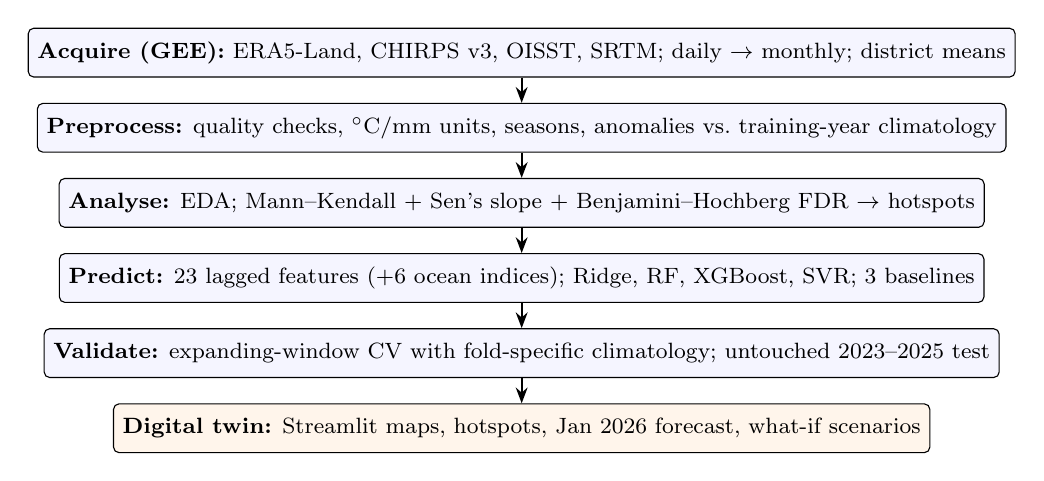
\begin{tikzpicture}[node distance=0.32cm, every node/.style={font=\footnotesize},
  box/.style={draw, rounded corners=2pt, align=center, minimum width=7.6cm, minimum height=0.62cm, fill=blue!4},
  arr/.style={-{Stealth[length=2mm]}, thick}]
\node[box] (a) {\textbf{Acquire (GEE):} ERA5-Land, CHIRPS v3, OISST, SRTM; daily $\rightarrow$ monthly; district means};
\node[box, below=of a] (b) {\textbf{Preprocess:} quality checks, \degC/mm units, seasons, anomalies vs.\ training-year climatology};
\node[box, below=of b] (c) {\textbf{Analyse:} EDA; Mann--Kendall + Sen's slope + Benjamini--Hochberg FDR $\rightarrow$ hotspots};
\node[box, below=of c] (d) {\textbf{Predict:} 23 lagged features (+6 ocean indices); Ridge, RF, XGBoost, SVR; 3 baselines};
\node[box, below=of d] (e) {\textbf{Validate:} expanding-window CV with fold-specific climatology; untouched 2023--2025 test};
\node[box, below=of e, fill=orange!8] (f) {\textbf{Digital twin:} Streamlit maps, hotspots, Jan 2026 forecast, what-if scenarios};
\foreach \x/\y in {a/b,b/c,c/d,d/e,e/f} \draw[arr] (\x) -- (\y);
\end{tikzpicture}
\caption{Pakistan ClimateTwin pipeline.}
\label{fig:pipeline}
\end{figure}

\subsection{Data Acquisition and Preprocessing}
For each month we average ERA5-Land \emph{daily} aggregates, so that monthly Tmax is the mean of daily maxima rather than the single hottest hour of the month, and sum daily CHIRPS rainfall. District means are computed with GEE \texttt{reduceRegions} at a 5\,km scale so that districts smaller than one ERA5-Land cell still receive values. Temperatures are converted from Kelvin to \degC, precipitation from metres to millimetres and radiation to MJ\,m$^{-2}$\,day$^{-1}$.

Quality checks covered row completeness (126 districts $\times$ 312 months), missing values, duplicates, the number of daily images per month and physically plausible ranges; all checks passed with zero failures. A within-district temporal interpolation routine handles interior gaps; no values required filling. For each variable $x$, district $d$, calendar month $m$ and year $y$, we compute the anomaly
\begin{equation}
a_{d,m,y} = x_{d,m,y} - \bar{x}_{d,m}, \qquad \bar{x}_{d,m} = \tfrac{1}{|Y|}\textstyle\sum_{y\in Y} x_{d,m,y},
\end{equation}
where the climatology period $Y$ contains \emph{training years only} (2000--2019). Anomalies remove the seasonal cycle and fixed geographic differences. Standardisation ($z$-scores) is applied inside each model pipeline and fitted on training rows only.

\subsection{Trend Analysis and Hotspots}
For each district we test the 26 annual means of Tmax, Tmin, Tmean, DTR (Tmax$-$Tmin) and annual rainfall with the non-parametric Mann--Kendall test~\cite{mann1945,kendall1975} and estimate trend magnitude with Sen's slope~\cite{sen1968}. Because 126 tests are run per variable, $p$-values are converted to Benjamini--Hochberg $q$-values~\cite{benjamini1995}. A district is a \emph{warming hotspot} if $q<0.05$ and the slope is positive. Elevation dependence is tested with the Spearman correlation between district elevation and Sen's slope.

\subsection{Forecasting Task and Features}
At the end of month $t$ we predict the Tmax anomaly of month $t+1$ for every district. We use anomalies rather than raw Tmax because raw temperature is almost perfectly explained by the seasonal cycle (Section~\ref{sec:r2}). Table~\ref{tab:features} lists the 23 features. All are computed from months $\le t$, except quantities known in advance (target calendar month, district attributes, climatology). Seasonal-persistence interactions allow linear models to use persistence that varies by season. The optional ocean group adds Ni\~{n}o-3.4~\cite{huang2021}, the Dipole Mode Index~\cite{saji1999} and tropical-mean (20$^\circ$S--20$^\circ$N) SST anomalies computed in GEE from OISST against a fixed 1982--2010 base, which ends before every validation and test year.

\begin{table}[t]
\centering
\caption{Feature groups (input month $t$; target month $t+1$)}
\label{tab:features}
\small
\begin{tabular}{@{}p{2.3cm}p{5.4cm}@{}}
\toprule
Group & Features \\
\midrule
Temperature memory & Tmax anomaly at $t$, $t-1$, $t-2$, 3-month mean; Tmin anomaly at $t$, $t-1$ \\
Moisture memory & rainfall anomaly at $t$, 3- and 6-month means; soil-moisture anomaly at $t$, $t-1$ \\
Radiation & net solar radiation anomaly at $t$ \\
Large-scale context & national mean Tmax anomaly at $t$ \\
Seasonal persistence & Tmax and national anomaly $\times$ sin/cos(target month) \\
Seasonality & sin/cos(target month); target-month Tmax climatology \\
Geography & elevation, latitude, longitude \\
\midrule
Ocean (optional) & Ni\~{n}o-3.4, DMI, tropical SST: value at $t$ and 3-month mean \\
\bottomrule
\end{tabular}
\end{table}

\subsection{Models and Baselines}
We compare four learners: Ridge regression~\cite{hoerl1970}, Random Forest (RF)~\cite{breiman2001}, XGBoost~\cite{chen2016} and $\varepsilon$-support vector regression (SVR) with an RBF kernel~\cite{drucker1997}, implemented with scikit-learn~\cite{pedregosa2011} and XGBoost. Three baselines are used: \emph{climatology} (anomaly $=0$), \emph{persistence} ($\hat a_{t+1}=a_t$) and \emph{damped persistence}, an AR(1) model $\hat a_{t+1}=\phi\,a_t$ with $\phi$ fitted by least squares on the training data ($\phi=0.31$).

\subsection{Validation Design}
Anomalies are strongly correlated across districts within a month, so a 3-year validation block contains only about 36 effective samples. We therefore tune hyperparameters with four \emph{expanding-window} folds inside 2000--2022 (validation blocks 2011--13, 2014--16, 2017--19 and 2020--22). Each fold trains only on earlier years. During development we found that using the global 2000--2019 climatology inside these folds leaks the validation-period mean into the training anomalies of folds 1--3. Each fold therefore \textbf{recomputes the climatology, all anomaly features and the target from its own training years}. Search spaces (grid search for Ridge, RF and SVR; 30-draw random search for XGBoost) were widened until every selected hyperparameter lay strictly inside its range. SVR is tuned on 8{,}000-row subsamples per fold for computational reasons. The selected configuration is refitted on 2000--2022 and evaluated once on the untouched 2023--2025 test set (4{,}536 district-months, 36 months).

\subsection{Evaluation}
We report MAE, RMSE, $R^2$, bias and the MSE skill score $\mathrm{SS}=1-\mathrm{MSE}_{\text{model}}/\mathrm{MSE}_{\text{ref}}$~\cite{murphy1988} against climatology and damped persistence. Uncertainty is quantified by a bootstrap~\cite{efron1993} that resamples whole \emph{months} (1{,}000 replicates), respecting spatial dependence. For extreme heat, a month is an event if its Tmax anomaly exceeds the training-period 90th percentile (1.76\,\degC). Each regressor's prediction is used as a score, with the F1-optimal threshold chosen on 2011--2022 out-of-fold predictions. Interpretability uses grouped permutation importance and SHAP~\cite{lundberg2017}. Spatial transferability is tested by leave-one-province-out (LOPO) refits for the five large provinces.

\subsection{Digital Twin}
A Streamlit dashboard reads pre-computed outputs and provides (i) interactive trend and climate maps with district histories, (ii) a January 2026 forecast from the best configuration refitted on 2000--2025, with an empirical 80\% error range, and model comparisons, and (iii) a scenario explorer that applies hypothetical temperature ($+0$ to $+3$\,\degC) and rainfall ($-30$ to $+20$\%) shifts to observed 2016--2025 months and recounts three heat-risk indicators (months $\ge$40\,\degC, locally extreme months, hot-and-dry months). Scenarios are explicitly labelled as hypothetical rather than projections.

% ---------------------------------------------------------------------
\section{Results}

\subsection{Temperature Trends and Hotspots (RQ1--RQ2)}
Nationally, annual Tmin rose by +0.19\,\degC/decade, Tmean by +0.06\,\degC/decade and Tmax showed no trend ($-0.02$\,\degC/decade, Mann--Kendall $p=0.93$; Fig.~\ref{fig:national}). The warmest years were 2025 and 2016. Tmin slopes are positive in 116 of 126 districts. The DTR decreased in 125 districts, significantly ($q<0.05$) in 44. Twelve districts are significant Tmin warming hotspots: six in Sindh (including Karachi and Hyderabad), four in Balochistan (Kech, Awaran, Gwadar, Lasbela; up to +0.44\,\degC/decade) and two in Khyber Pakhtunkhwa (Abbottabad, Mardan). Without FDR correction, 42 districts would have been declared significant, which illustrates the importance of multiple-testing control. No district has a significant Tmax trend after correction (Fig.~\ref{fig:trendmaps}).

\begin{figure}[t]
\centering
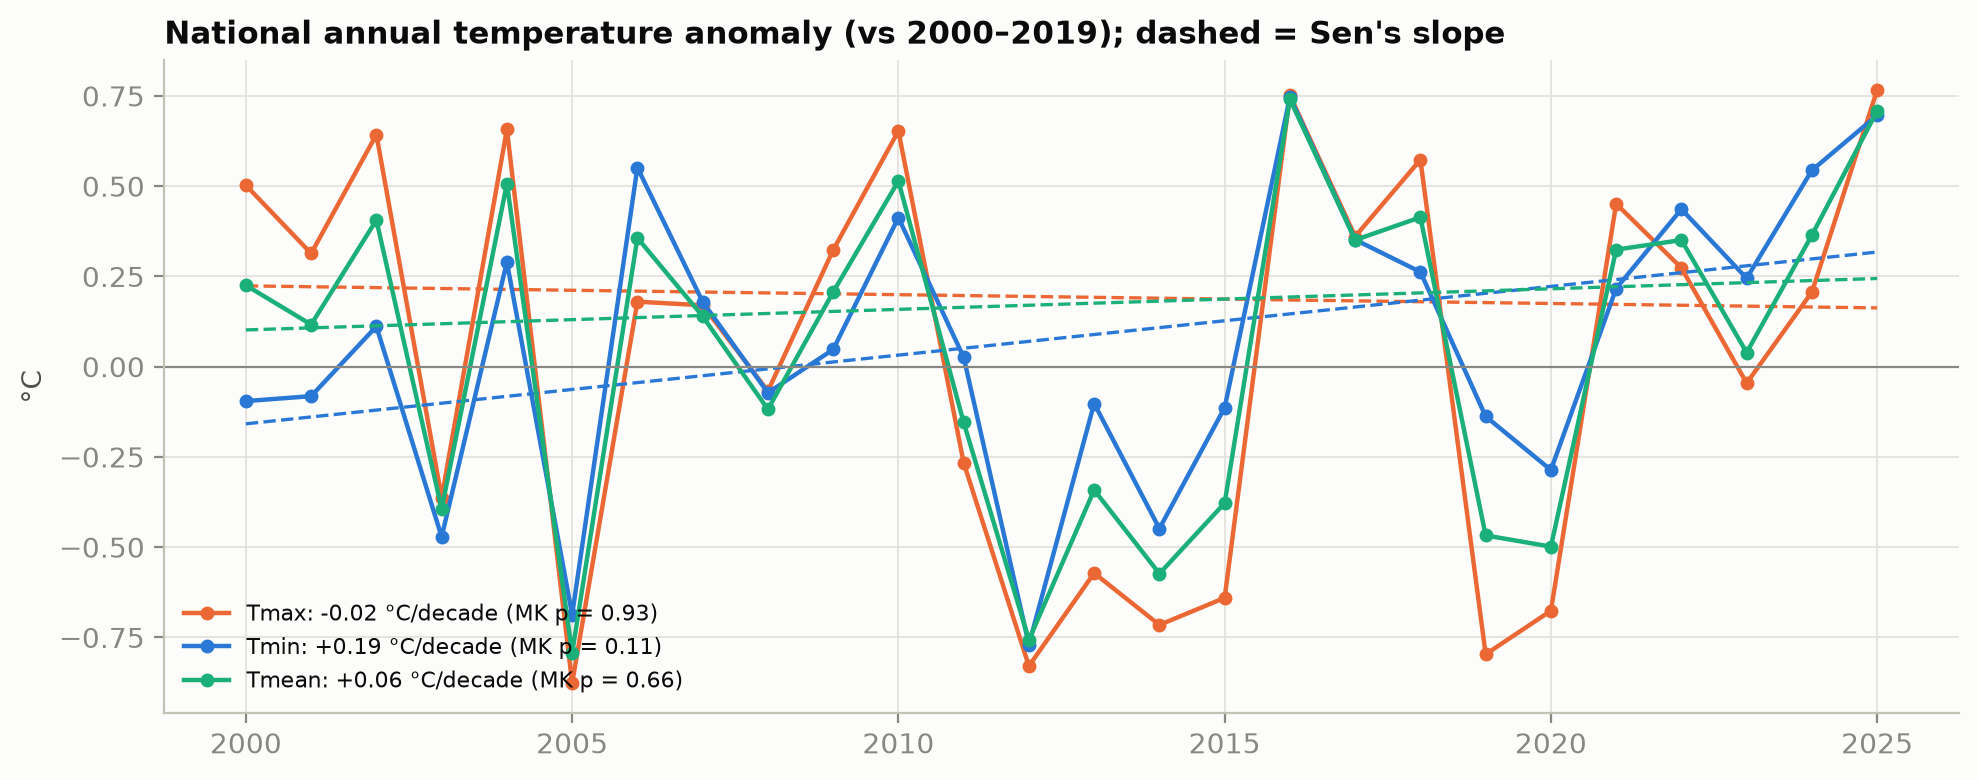
\includegraphics[width=\columnwidth]{eda_03_national_trend.png}
\caption{National annual temperature anomalies (vs.\ 2000--2019) with Sen's slope lines.}
\label{fig:national}
\end{figure}

\begin{figure*}[t]
\centering
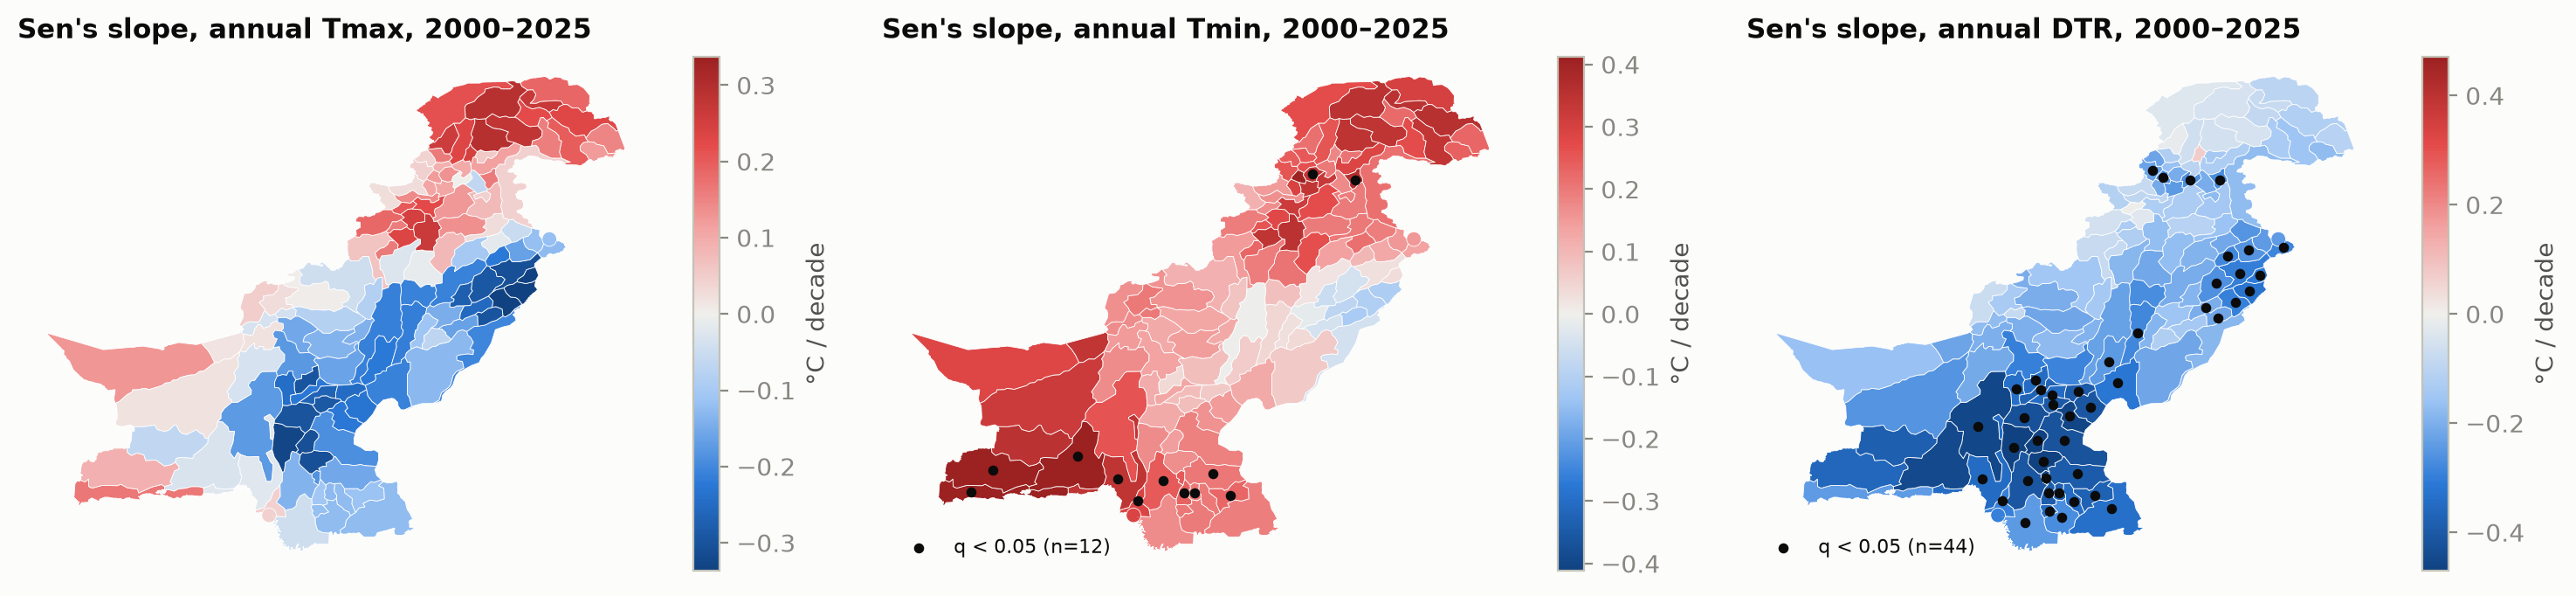
\includegraphics[width=\textwidth]{eda_05_trend_maps.png}
\caption{Sen's slope of annual Tmax, Tmin and diurnal temperature range (DTR), 2000--2025. Dots mark districts significant after Benjamini--Hochberg correction ($q<0.05$).}
\label{fig:trendmaps}
\end{figure*}

\textit{Seasonality.} Monsoon-season (JJAS) Tmin shows the strongest signal: +0.34\,\degC/decade nationally ($p=0.001$), significant after FDR in 85 districts. Pre-monsoon (MAM) Tmax shows a broad but non-significant cooling across the plains.

\textit{Elevation.} District Tmax trends increase with elevation (Spearman $\rho=0.69$, $p<0.001$; Fig.~\ref{fig:edw}). Gilgit-Baltistan and upper Khyber Pakhtunkhwa warm by about +0.15 to +0.30\,\degC/decade, whereas the plains of Punjab and Sindh show daytime cooling of up to $-0.4$\,\degC/decade, consistent with EDW~\cite{pepin2015}.

\begin{figure}[t]
\centering
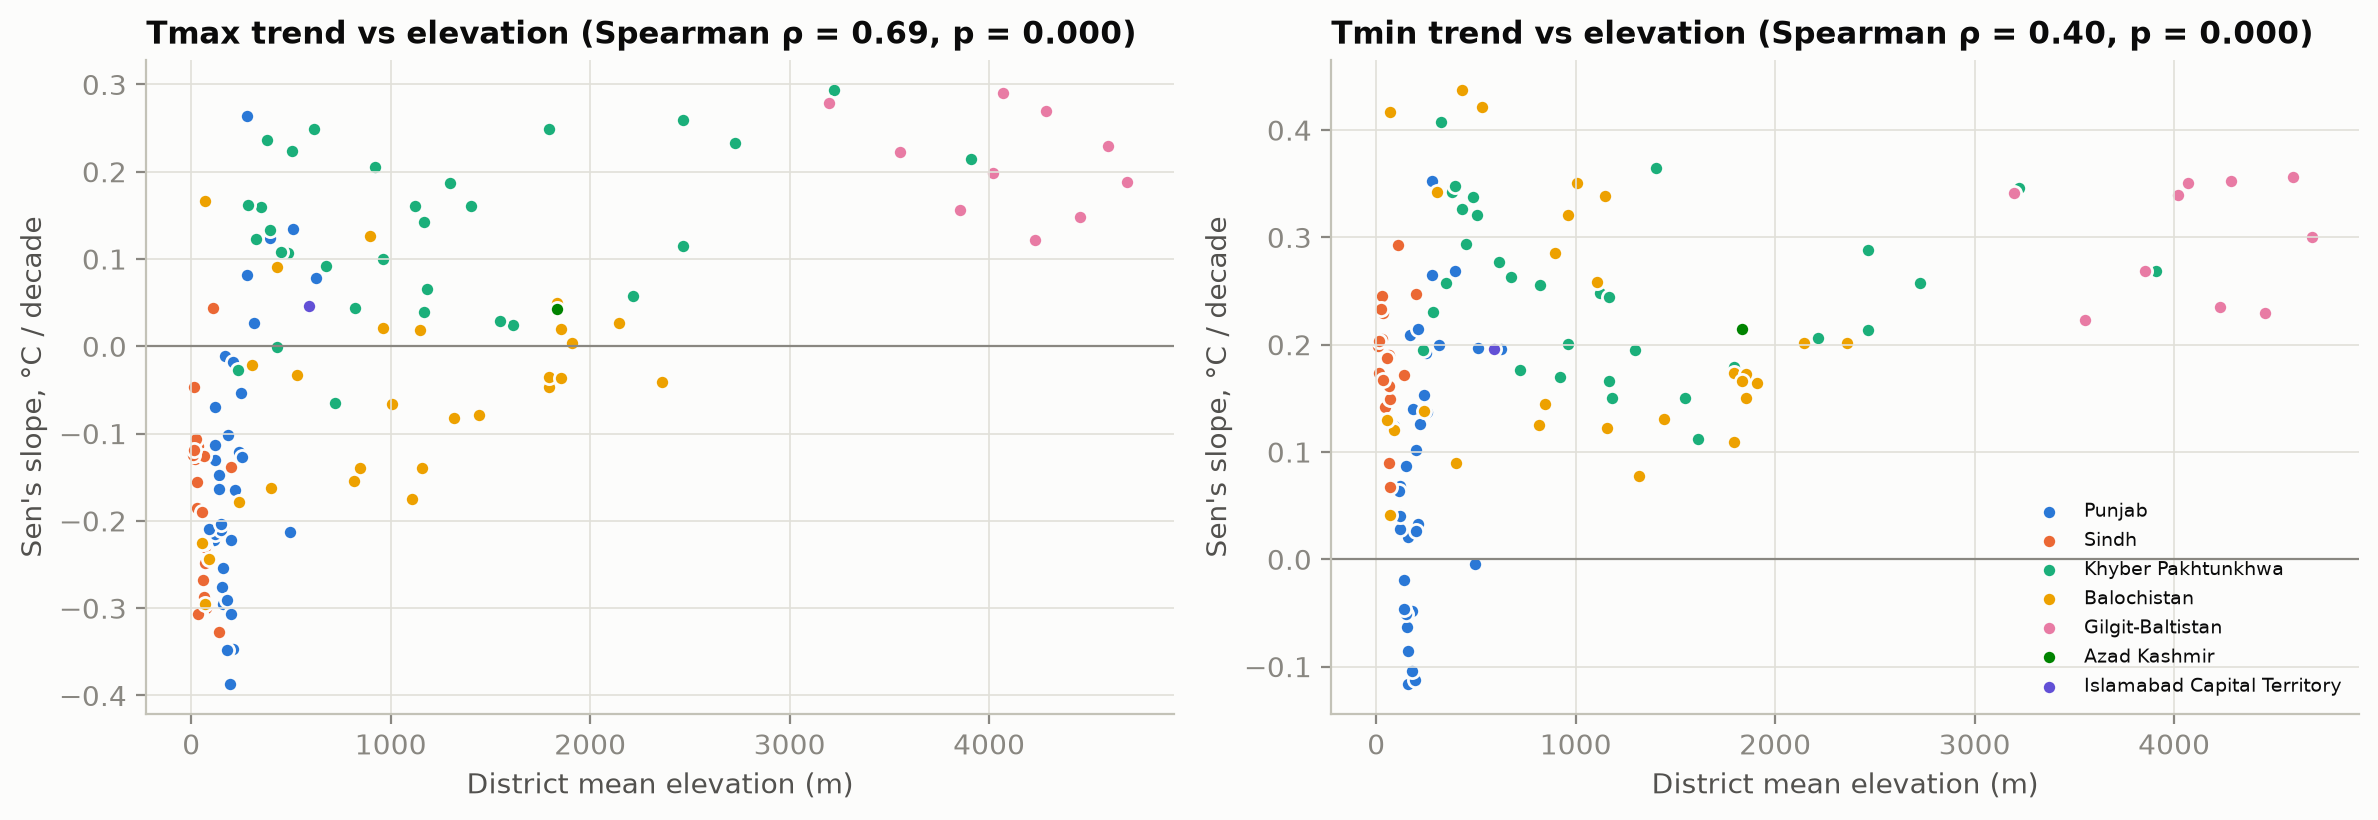
\includegraphics[width=\columnwidth]{eda_07_elevation_dependence.png}
\caption{District Sen's slope versus mean elevation for Tmax (left) and Tmin (right), coloured by province.}
\label{fig:edw}
\end{figure}

\subsection{Rainfall and Temperature (RQ3)}
Mean district rainfall increased by +49\,mm/decade (Mann--Kendall $p=0.043$), but only three districts are significant after FDR correction. In every season, wetter-than-normal months are cooler by day (Spearman $\rho$ between rainfall and Tmax anomalies from $-0.31$ to $-0.54$; soil moisture $-0.54$ to $-0.77$), while Tmin is largely unaffected. ERA5-Land precipitation exceeds CHIRPS by +10.2\,mm/month (+28\%) on average, so the gauge-corrected CHIRPS is used as the primary rainfall source.

\subsection{Cross-Validated Model Comparison (RQ4--RQ5)}
Table~\ref{tab:cv} shows the leakage-free CV results. All tuned models beat climatology and raw persistence, but none beats damped persistence on average. Tuning consistently selected strong regularisation: Ridge $\alpha=10^4$, RF with depth 4 and at least 100 samples per leaf, XGBoost with depth-1 trees, and SVR with $C=0.1$. A Ridge feature ablation showed that only the seasonal-persistence group clearly helps ($+0.006$\,\degC RMSE when removed).

\begin{table}[t]
\centering
\caption{Expanding-window CV RMSE (\degC) by validation block}
\label{tab:cv}
\small
\begin{tabular}{@{}lccccc@{}}
\toprule
Model & 11--13 & 14--16 & 17--19 & 20--22 & Mean \\
\midrule
Climatology & 1.563 & 1.620 & 1.467 & 1.875 & 1.631 \\
Persistence & 1.730 & 1.696 & 1.769 & 2.024 & 1.805 \\
Damped persistence & 1.462 & \textbf{1.499} & 1.401 & \textbf{1.718} & \textbf{1.520} \\
\midrule
Ridge & 1.480 & 1.512 & 1.375 & 1.758 & 1.531 \\
Random Forest & 1.496 & 1.512 & 1.358 & 1.790 & 1.539 \\
XGBoost & 1.484 & 1.529 & 1.357 & 1.811 & 1.545 \\
SVR & \textbf{1.457} & 1.514 & \textbf{1.339} & 1.803 & 1.528 \\
\bottomrule
\end{tabular}
\end{table}

\subsection{Test-Set Performance}
On 2023--2025 (Table~\ref{tab:test}), Ridge is the best local-feature model (RMSE 1.673\,\degC, +9.1\% skill vs.\ climatology, +1.8\% vs.\ damped persistence). RF, XGBoost and SVR are slightly worse than damped persistence. However, the 95\% month-bootstrap intervals of all ML skill scores include zero against both references (Fig.~\ref{fig:ci}); only raw persistence is significantly worse than damped persistence. Skill is highest for pre-monsoon and monsoon targets and close to zero in winter. Ridge beats climatology in 118 of 126 districts. All models under-predict the warm test period (mean actual anomaly +0.31\,\degC; bias $-0.26$ to $-0.33$\,\degC) and strongly shrink extreme anomalies.

\begin{table}[t]
\centering
\caption{Test results, 2023--2025 (MSE skill in \%)}
\label{tab:test}
\small
\begin{tabular}{@{}lcccc@{}}
\toprule
Model & RMSE & Skill vs.\ & Skill vs.\ & Bias \\
 & (\degC) & clim. & damped & (\degC) \\
\midrule
Climatology & 1.756 & 0.0 & $-8.0$ & $-0.31$ \\
Persistence & 2.095 & $-42.4$ & $-53.9$ & $-0.04$ \\
Damped persistence & 1.689 & 7.4 & 0.0 & $-0.22$ \\
\midrule
Ridge & 1.673 & 9.1 & 1.8 & $-0.29$ \\
Random Forest & 1.711 & 5.0 & $-2.6$ & $-0.27$ \\
XGBoost & 1.695 & 6.8 & $-0.7$ & $-0.26$ \\
SVR & 1.706 & 5.6 & $-2.0$ & $-0.33$ \\
\midrule
Ridge + ocean & \textbf{1.650} & \textbf{11.7} & \textbf{4.6} & $-0.23$ \\
\bottomrule
\end{tabular}
\end{table}

\begin{figure*}[t]
\centering
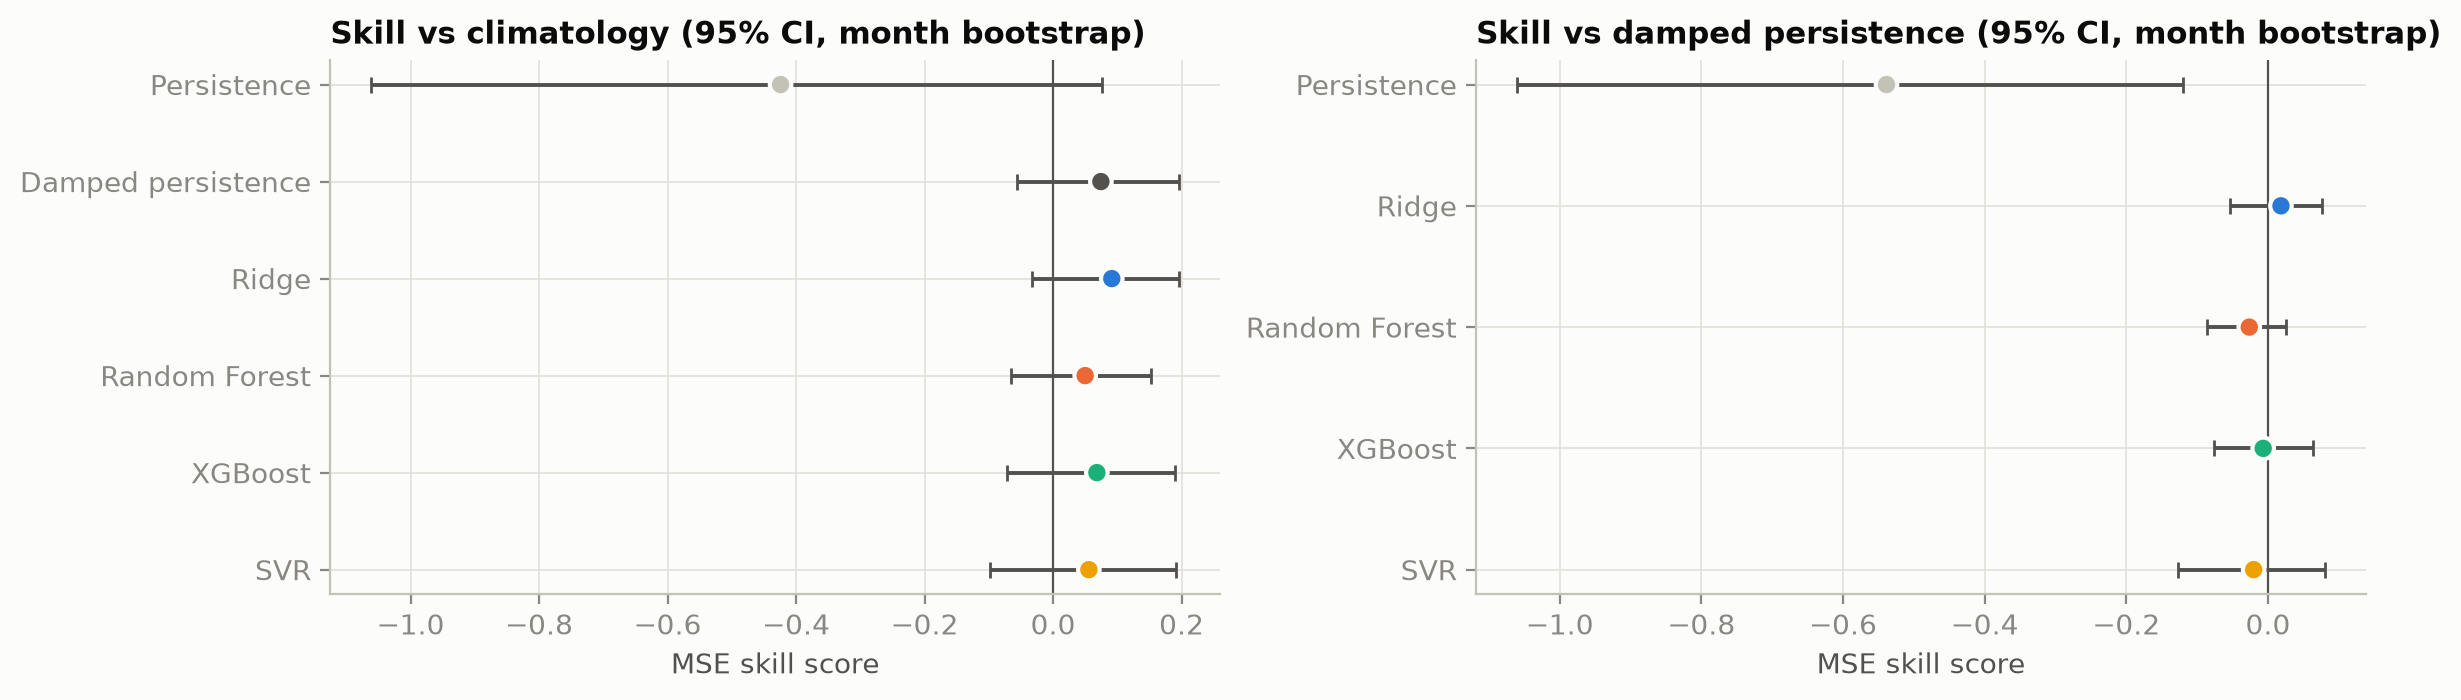
\includegraphics[width=0.92\textwidth]{ml_03_skill_ci.png}
\caption{Test-set MSE skill scores relative to climatology (left) and damped persistence (right), with 95\% confidence intervals from a month-block bootstrap.}
\label{fig:ci}
\end{figure*}

\textit{Extreme-heat months.} The event rate rose from 9.6\% in 2011--2022 to 18.2\% in the test period. With out-of-fold thresholds, Ridge and SVR reach F1 $=0.37$ (precision 0.28--0.30, recall 0.51--0.58), compared with 0.31 for damped persistence. PR-AUC is 0.24--0.27 against a no-skill level of 0.18. ML therefore adds more value for flagging extremes than for average error.

\subsection{Why Raw-Temperature $R^2$ Misleads}\label{sec:r2}
When climatology is added back to the predicted anomaly, every method, including the climatology baseline itself, reaches $R^2\approx0.98$ on raw Tmax, while $R^2$ on the anomaly target ranges from $-0.03$ to $0.06$. High raw-temperature $R^2$ therefore says little about forecasting skill.

\subsection{Drivers of Predictability}
Grouped permutation importance and SHAP (Fig.~\ref{fig:shap}) agree that the solar-radiation anomaly is the strongest predictor (clear-sky months tend to precede warm months), followed by temperature memory and the national anomaly. Geography contributes nothing, as expected for anomalies. The seasonal-persistence interactions, which helped in CV, have negative permutation importance on the test set, a reminder that small CV gains in weak-signal problems may not generalise.

\begin{figure}[t]
\centering
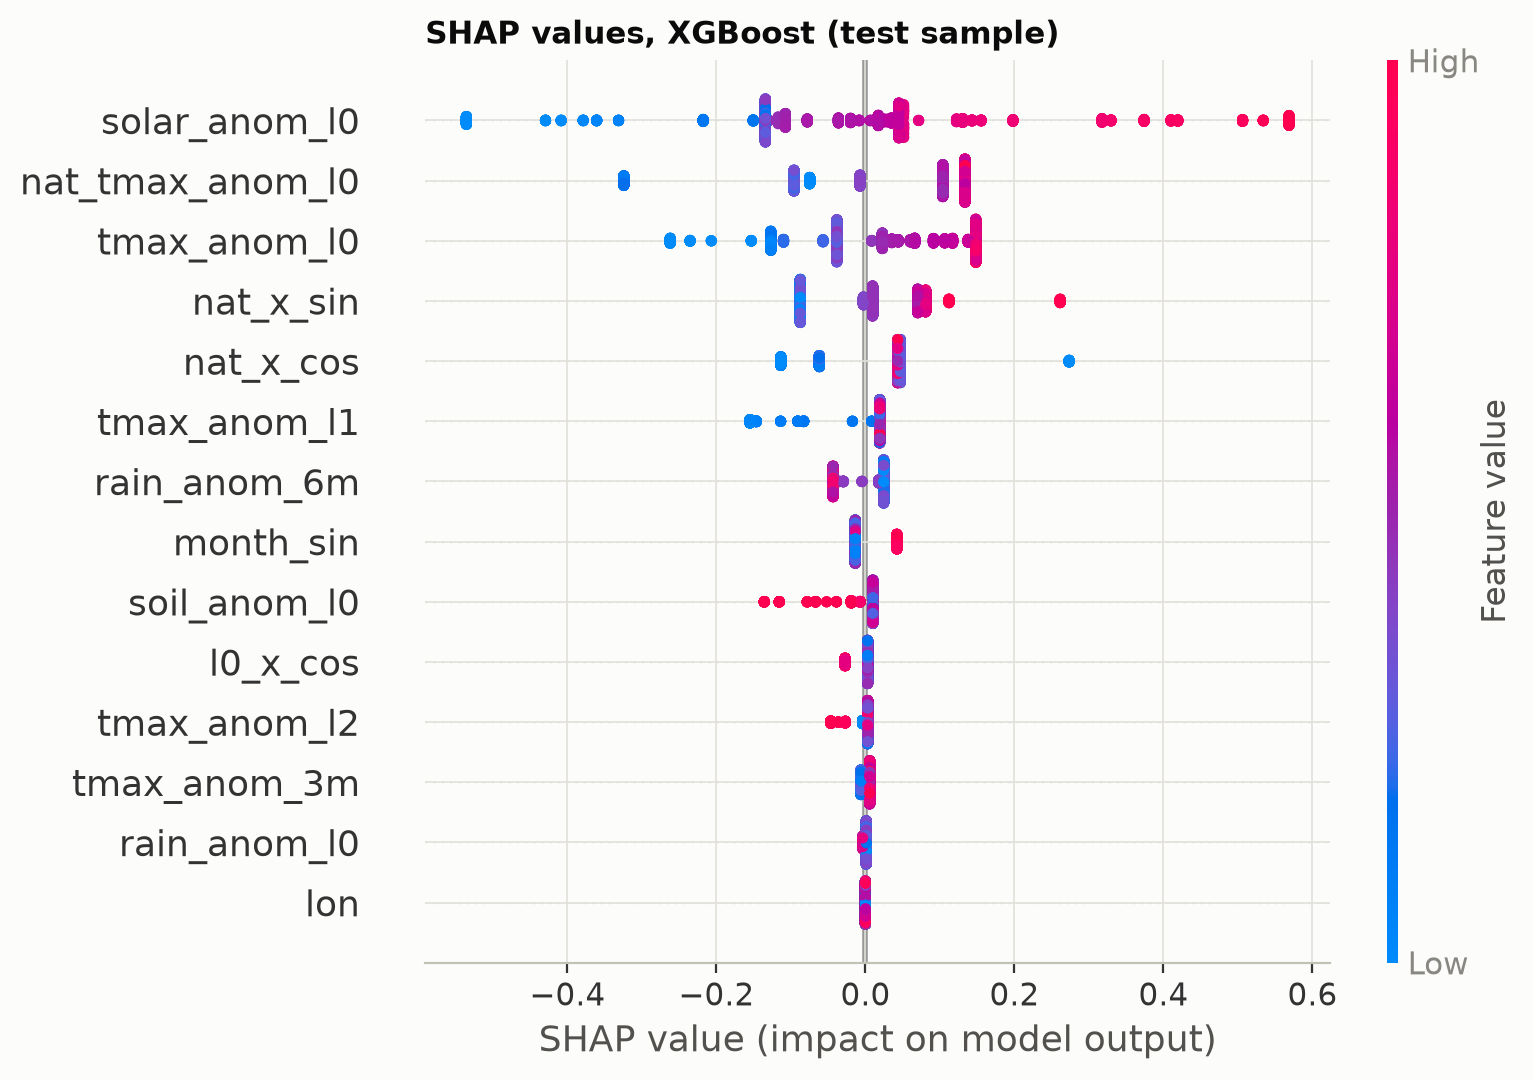
\includegraphics[width=\columnwidth]{ml_11_shap_summary.png}
\caption{SHAP summary for XGBoost on a 3{,}000-row test sample.}
\label{fig:shap}
\end{figure}

\subsection{Spatial Transferability}
In the LOPO experiment, skill drops by at most 0.015 on average (Ridge: 0.002) when a province is excluded from training (Fig.~\ref{fig:lopo}). The learned relationships, chiefly persistence and radiation, therefore transfer across regions. Skill is highest in Khyber Pakhtunkhwa and Gilgit-Baltistan and lowest in Sindh.

\begin{figure*}[t]
\centering
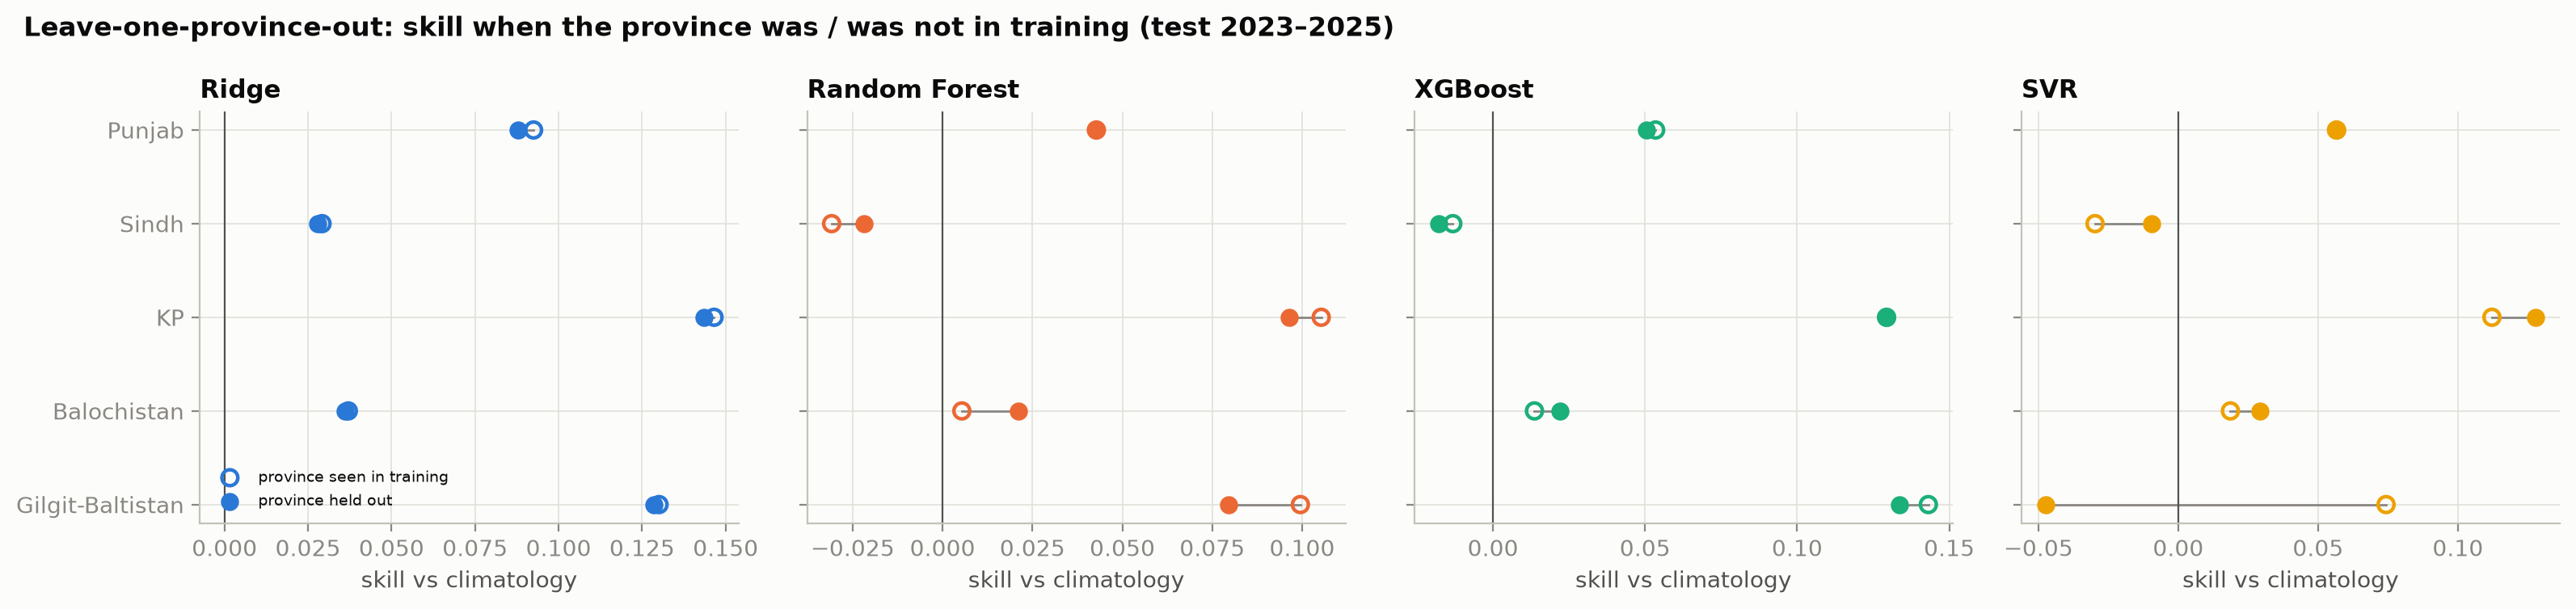
\includegraphics[width=\textwidth]{ml_13_lopo.png}
\caption{Leave-one-province-out: test skill when the province was seen in training (open) versus held out (filled).}
\label{fig:lopo}
\end{figure*}

\subsection{Ocean Drivers (RQ6)}
In the training years, no district shows an FDR-significant correlation between Tmax and ENSO or IOD, in the same month or one month ahead. National-level links exist for some seasons, e.g., Ni\~{n}o-3.4 at $t$ versus post-monsoon Tmax at $t+1$ ($\rho=-0.49$). After retuning all models with the ocean indices, CV changes little (Ridge $-0.002$\,\degC; tree models and SVR $+0.009$ to $+0.015$\,\degC). On the test set, however, all four models improve (Fig.~\ref{fig:ocean}). Ridge + ocean reaches RMSE 1.650\,\degC and +11.7\% skill vs.\ climatology, a significant gain over local Ridge (+2.8\%, 95\% CI [+0.04\%, +5.8\%]) but not significant against damped persistence (+4.6\%, CI [$-1.7$\%, +10.5\%]). The ocean indices mainly reduce the warming bias (e.g., XGBoost $-0.26\rightarrow-0.13$\,\degC), because tropical SST tracks background warming.

\begin{figure*}[t]
\centering
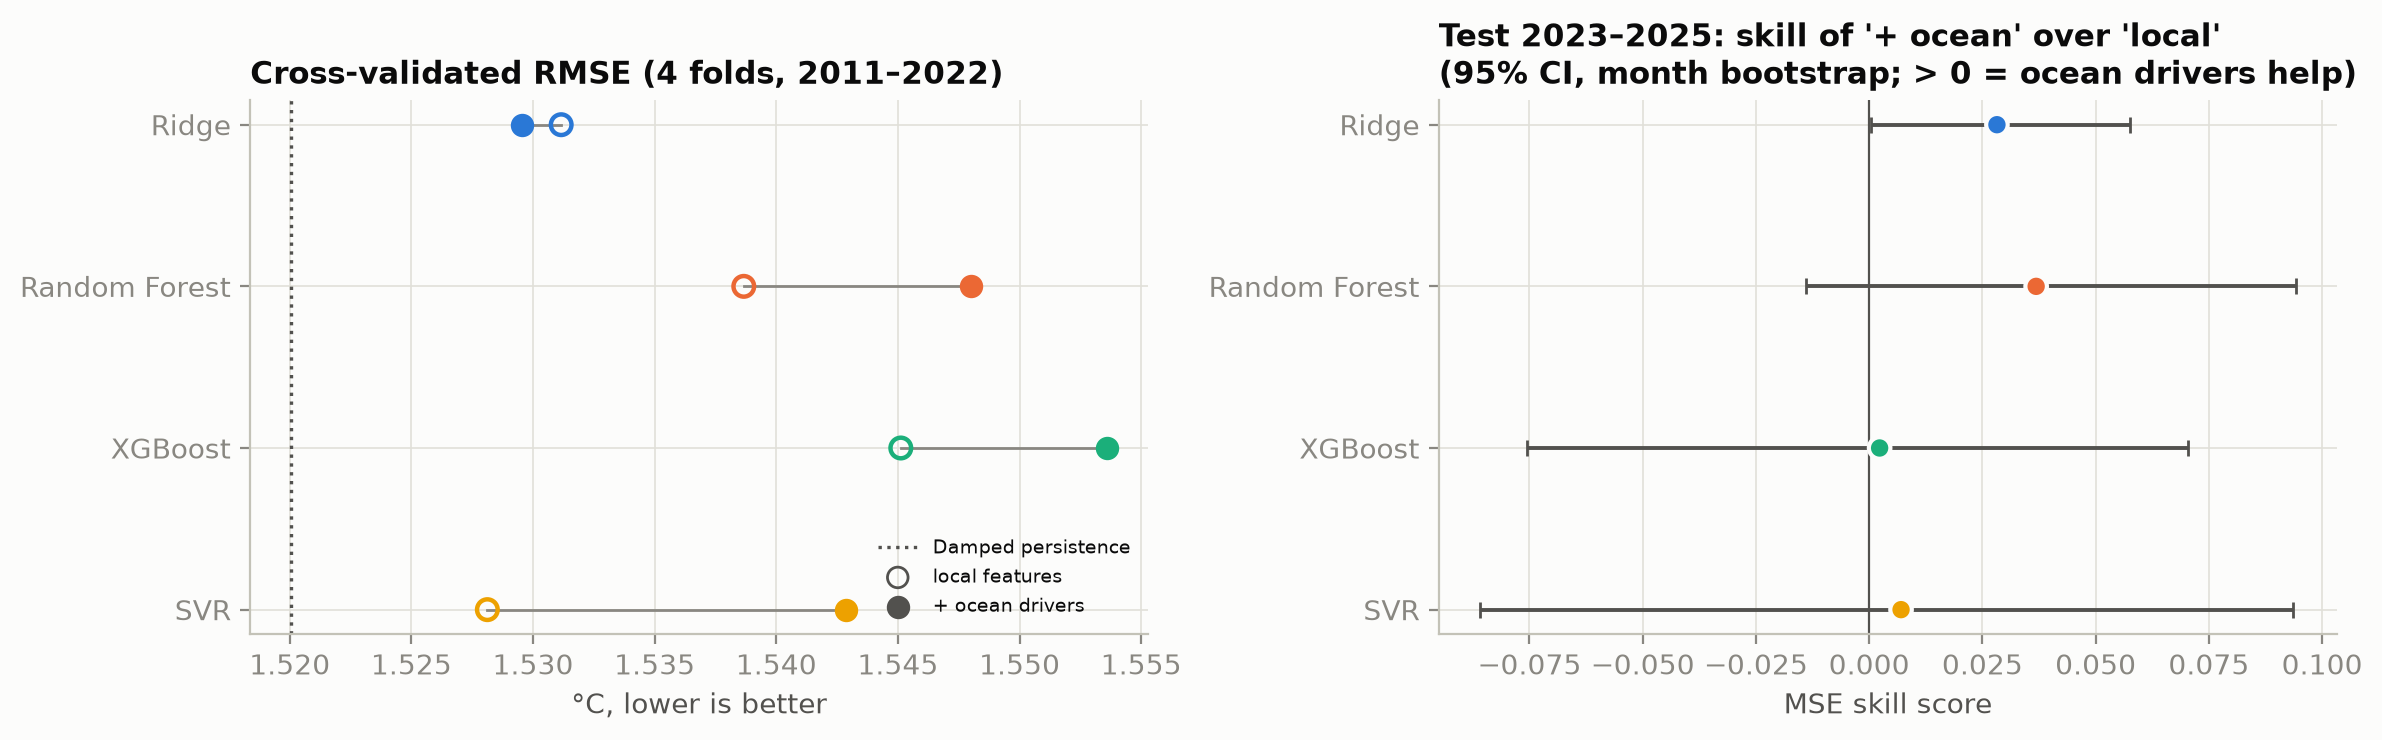
\includegraphics[width=0.92\textwidth]{oc_03_ocean_vs_local.png}
\caption{Effect of ocean drivers. Left: CV RMSE with local features (open) and with ocean indices (filled). Right: test-set skill of ``+ ocean'' over ``local'' with 95\% month-bootstrap CIs.}
\label{fig:ocean}
\end{figure*}

% ---------------------------------------------------------------------
\section{Discussion}
\textit{Night-time, monsoon-season warming.} The dominance of Tmin warming and the shrinking DTR agree with global findings~\cite{vose2005}. Contrasting daytime trends between mountains and irrigated plains are consistent with EDW~\cite{pepin2015} and with irrigation-induced surface cooling and moistening~\cite{mishra2020}. We do not test these mechanisms directly; they are hypotheses for future attribution work. Our Tmax result differs from station studies reporting widespread Tmax increases over earlier periods~\cite{iqbal2016}. Differences in period (2000--2025 vs.\ from the 1950s), reanalysis versus station data and spatial aggregation could each contribute.

\textit{Limits of predictability.} One month ahead, district Tmax anomalies are weakly predictable: the best configuration explains about 12\% of anomaly variance relative to climatology, and the differences between learners are smaller than sampling uncertainty over 36 test months. Hyperparameter tuning consistently chose the simplest models, and a regularised linear model performed best. These results argue for reporting skill against strong baselines with honest uncertainty, rather than raw-temperature accuracy.

\textit{Non-stationarity.} All models under-predict the warmer test years. Indices that track background ocean warming reduce this bias, which explains why ocean drivers help on 2023--2025 but not in earlier CV blocks. Tree ensembles cannot extrapolate trending predictors beyond their training range, which partly explains their weaker response.

\textit{Limitations.} ERA5-Land is a reanalysis rather than station data; district means hide intra-district variability; the 126-unit boundary set is outdated; the test period contains only 36 months; and scenario results are hypothetical, not projections.

% ---------------------------------------------------------------------
\section{Conclusion}
Pakistan ClimateTwin combines GEE data, statistical trend analysis and ML in an interactive digital twin for 126 districts. Between 2000 and 2025, warming in Pakistan was mainly a night-time and monsoon-season phenomenon, with hotspots in Sindh and coastal Balochistan and elevation-dependent daytime trends. Next-month heat is only weakly predictable from local predictors. Ridge regression with ENSO, IOD and tropical-SST indices performs best (+11.7\% skill over climatology), while more complex models do not beat a damped-persistence baseline. Future work includes sub-monthly lead times, explicit trend-aware models, station-based validation and attribution of the irrigation and elevation signals.

% ---------------------------------------------------------------------
\section*{Code and Data Availability}
Code, notebooks and the dashboard are available in the project repository [link to be added]. The processed dataset is available at [link to be added] and can be regenerated with the included GEE scripts.

% ---------------------------------------------------------------------
\begin{thebibliography}{00}
\bibitem{delrio2013} S. del R\'{i}o \textit{et al.}, ``Recent mean temperature trends in Pakistan and links with teleconnection patterns,'' \textit{Int. J. Climatol.}, vol. 33, no. 2, pp. 277--290, 2013, doi: 10.1002/joc.3423.
\bibitem{iqbal2016} M. A. Iqbal, A. Penas, A. Cano-Ortiz, K. C. Kersebaum, L. Herrero, and S. del R\'{i}o, ``Analysis of recent changes in maximum and minimum temperatures in Pakistan,'' \textit{Atmos. Res.}, vol. 168, pp. 234--249, 2016, doi: 10.1016/j.atmosres.2015.09.016.
\bibitem{vose2005} R. S. Vose, D. R. Easterling, and B. Gleason, ``Maximum and minimum temperature trends for the globe: An update through 2004,'' \textit{Geophys. Res. Lett.}, vol. 32, no. 23, 2005, doi: 10.1029/2005GL024379.
\bibitem{pepin2015} N. Pepin \textit{et al.}, ``Elevation-dependent warming in mountain regions of the world,'' \textit{Nature Climate Change}, vol. 5, no. 5, pp. 424--430, 2015, doi: 10.1038/nclimate2563.
\bibitem{mishra2020} V. Mishra \textit{et al.}, ``Moist heat stress extremes in India enhanced by irrigation,'' \textit{Nature Geosci.}, vol. 13, no. 11, pp. 722--728, 2020, doi: 10.1038/s41561-020-00650-8.
\bibitem{saji1999} N. H. Saji, B. N. Goswami, P. N. Vinayachandran, and T. Yamagata, ``A dipole mode in the tropical Indian Ocean,'' \textit{Nature}, vol. 401, pp. 360--363, 1999, doi: 10.1038/43854.
\bibitem{hussain2024} A. Hussain \textit{et al.}, ``Increasing monsoon precipitation extremes in relation to large-scale climatic patterns in Pakistan,'' \textit{Atmos. Res.}, vol. 309, Art. no. 107592, 2024, doi: 10.1016/j.atmosres.2024.107592.
\bibitem{munoz2021} J. Mu\~{n}oz-Sabater \textit{et al.}, ``ERA5-Land: A state-of-the-art global reanalysis dataset for land applications,'' \textit{Earth Syst. Sci. Data}, vol. 13, no. 9, pp. 4349--4383, 2021, doi: 10.5194/essd-13-4349-2021.
\bibitem{funk2015} C. Funk \textit{et al.}, ``The climate hazards infrared precipitation with stations---a new environmental record for monitoring extremes,'' \textit{Sci. Data}, vol. 2, Art. no. 150066, 2015, doi: 10.1038/sdata.2015.66.
\bibitem{funk2026} C. Funk \textit{et al.}, ``The Climate Hazards Center Infrared Precipitation with Stations, Version 3,'' \textit{Sci. Data}, vol. 13, Art. no. 718, 2026, doi: 10.1038/s41597-026-07096-4.
\bibitem{huang2021} B. Huang \textit{et al.}, ``Improvements of the Daily Optimum Interpolation Sea Surface Temperature (DOISST) Version 2.1,'' \textit{J. Climate}, vol. 34, no. 8, pp. 2923--2939, 2021, doi: 10.1175/JCLI-D-20-0166.1.
\bibitem{farr2007} T. G. Farr \textit{et al.}, ``The Shuttle Radar Topography Mission,'' \textit{Rev. Geophys.}, vol. 45, no. 2, 2007, doi: 10.1029/2005RG000183.
\bibitem{runfola2020} D. Runfola \textit{et al.}, ``geoBoundaries: A global database of political administrative boundaries,'' \textit{PLoS ONE}, vol. 15, no. 4, Art. no. e0231866, 2020, doi: 10.1371/journal.pone.0231866.
\bibitem{gorelick2017} N. Gorelick, M. Hancher, M. Dixon, S. Ilyushchenko, D. Thau, and R. Moore, ``Google Earth Engine: Planetary-scale geospatial analysis for everyone,'' \textit{Remote Sens. Environ.}, vol. 202, pp. 18--27, 2017, doi: 10.1016/j.rse.2017.06.031.
\bibitem{bauer2021} P. Bauer, B. Stevens, and W. Hazeleger, ``A digital twin of Earth for the green transition,'' \textit{Nature Climate Change}, vol. 11, no. 2, pp. 80--83, 2021, doi: 10.1038/s41558-021-00986-y.
\bibitem{mann1945} H. B. Mann, ``Nonparametric tests against trend,'' \textit{Econometrica}, vol. 13, no. 3, pp. 245--259, 1945.
\bibitem{kendall1975} M. G. Kendall, \textit{Rank Correlation Methods}, 4th ed. London, U.K.: Charles Griffin, 1975.
\bibitem{sen1968} P. K. Sen, ``Estimates of the regression coefficient based on Kendall's tau,'' \textit{J. Amer. Statist. Assoc.}, vol. 63, no. 324, pp. 1379--1389, 1968.
\bibitem{benjamini1995} Y. Benjamini and Y. Hochberg, ``Controlling the false discovery rate: A practical and powerful approach to multiple testing,'' \textit{J. Roy. Statist. Soc. B}, vol. 57, no. 1, pp. 289--300, 1995.
\bibitem{roberts2017} D. R. Roberts \textit{et al.}, ``Cross-validation strategies for data with temporal, spatial, hierarchical, or phylogenetic structure,'' \textit{Ecography}, vol. 40, no. 8, pp. 913--929, 2017, doi: 10.1111/ecog.02881.
\bibitem{bergmeir2012} C. Bergmeir and J. M. Ben\'{i}tez, ``On the use of cross-validation for time series predictor evaluation,'' \textit{Inf. Sci.}, vol. 191, pp. 192--213, 2012.
\bibitem{murphy1988} A. H. Murphy, ``Skill scores based on the mean square error and their relationships to the correlation coefficient,'' \textit{Mon. Weather Rev.}, vol. 116, no. 12, pp. 2417--2424, 1988.
\bibitem{efron1993} B. Efron and R. J. Tibshirani, \textit{An Introduction to the Bootstrap}. New York, NY, USA: Chapman \& Hall, 1993.
\bibitem{hoerl1970} A. E. Hoerl and R. W. Kennard, ``Ridge regression: Biased estimation for nonorthogonal problems,'' \textit{Technometrics}, vol. 12, no. 1, pp. 55--67, 1970.
\bibitem{breiman2001} L. Breiman, ``Random forests,'' \textit{Mach. Learn.}, vol. 45, no. 1, pp. 5--32, 2001.
\bibitem{chen2016} T. Chen and C. Guestrin, ``XGBoost: A scalable tree boosting system,'' in \textit{Proc. 22nd ACM SIGKDD Int. Conf. Knowl. Discov. Data Mining}, 2016, pp. 785--794.
\bibitem{drucker1997} H. Drucker, C. J. C. Burges, L. Kaufman, A. Smola, and V. Vapnik, ``Support vector regression machines,'' in \textit{Adv. Neural Inf. Process. Syst. 9}, 1997, pp. 155--161.
\bibitem{pedregosa2011} F. Pedregosa \textit{et al.}, ``Scikit-learn: Machine learning in Python,'' \textit{J. Mach. Learn. Res.}, vol. 12, pp. 2825--2830, 2011.
\bibitem{lundberg2017} S. M. Lundberg and S.-I. Lee, ``A unified approach to interpreting model predictions,'' in \textit{Adv. Neural Inf. Process. Syst. 30}, 2017, pp. 4765--4774.
\end{thebibliography}

\end{document}
